\subsection{Edge}

\begin{multicols}{2}
El filtro EDGE devuelve una imagen con los bordes de otra imagen original. Esto se logra observando los pixeles donde la intensidad de la imagen cambia de forma abrupta, lo cual puede ser logrado buscando saltos en una función de intensidades. Esta idea de detectar los bordes fue implementada a través del operador de Laplace, cuya matriz es: 

$$ M = \left(
\begin{matrix}
    0.5 & 1 & 0.5 \\
    1 & -6 & 1 \\
    0.5 & 1 & 0.5
\end{matrix}
\right)$$

\begin{center}
	\begin{tabular}{cccc}
		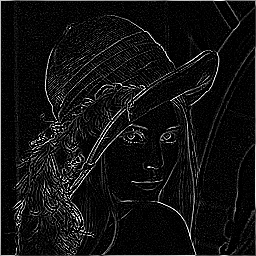
\includegraphics[width=0.3\textwidth]{imagenes/lenaEDGA.jpg} \\
		\end{tabular}
	\end{center}
\end{multicols}

La forma de utilizarla es posicionando uno a uno cada pixel en el centro de la matriz y realizando el siguiente cálculo: 

$$dst(x, y) = \sum_{k = 0}^2 \sum_{l = 0}^2 src(x + k - 1, y + l - 1) * M(k, l)$$

Al igual que monocromatizar, EDGE opera sobre imágenes en escala de grises (1 componente de color por píxel).
Como no se pueden procesar los bordes con la función anterior se aplica la siguiente función: $dst(x, y) = src(x,y)$.

\subsubsection{Implementación C}

Ignorando la primera y la última fila al igual que el primer y el último pixel de cada fila, recorrimos iterativamente todos los pixeles de la imagen realizando el siguiente proceso: por cada pixel calculamos todas las sumas parciales de la función que resulta de la aplicación de la matriz de Laplace, luego todas estas sumas fueron almacenadas en una variable auxiliar (\textit{edge}). Si el valor de \textit{edge} requería ser saturado se lo restringió a los valores 0/255 y finalmente se guardó el resultado en el pixel correspondiente de la imagen destino.

\begin{algorithm}[H]
  \begin{algorithmic}[1]
		\FORALL{y:=1 \TO  Height($I_{src}$$-1$)}
			\FORALL{x:=1 \TO  Width($I_{src}$)$-1$}
			  \STATE $m_{0,0} \gets I_{src}(x-1,y-1)*0.5$
			  \STATE $m_{0,1} \gets I_{src}(x-1,y)*1$
			  \STATE $m_{0,2} \gets I_{src}(x-1,y+1)*0.5$
			  \STATE $m_{1,0} \gets I_{src}(x,y-1)*1$
			  \STATE $m_{1,1} \gets I_{src}(x,y)*(-6)$
			  \STATE $m_{1,2} \gets I_{src}(x,y+1)*1$
			  \STATE $m_{2,0} \gets I_{src}(x+1,y-1)*0.5$
			  \STATE $m_{2,1} \gets I_{src}(x+1,y)*1$
			  \STATE $m_{2,2} \gets I_{src}(x+1,y+1)*0.5$
			  \STATE $edge \gets m_{0,0}+m_{0,1}+m_{0,2}+m_{1,0}+m_{1,1}+m_{1,2}+m_{2,0}+m_{2,1}+m_{2,2}$
			  \STATE $I_{dst}(x,y) \gets Saturar(edge)$
			\ENDFOR
		 \ENDFOR
  \end{algorithmic}
  \caption{$edge (I_{src}, I_{dst})$}
  \label{alg:edge}
\end{algorithm}

\subsubsection{Implementación ASM}